% ****** Start of file apssamp.tex ******
%
%   This file is part of the APS files in the REVTeX 4.2 distribution.
%   Version 4.2a of REVTeX, December 2014
%
%   Copyright (c) 2014 The American Physical Society.
%
%   See the REVTeX 4 README file for restrictions and more information.
%
% TeX'ing this file requires that you have AMS-LaTeX 2.0 installed
% as well as the rest of the prerequisites for REVTeX 4.2
%
% See the REVTeX 4 README file
% It also requires running BibTeX. The commands are as follows:
%
%  1)  latex apssamp.tex
%  2)  bibtex apssamp
%  3)  latex apssamp.tex
%  4)  latex apssamp.tex
%
\documentclass[superscriptaddress,unsortedaddress,
%runinaddress,
%frontmatterverbose, 
%preprint,
%preprintnumbers,
%nofootinbib,
%nobibnotes,
%bibnotes,
 amsmath,amssymb,
 aps,
%pra,
%prb,
%rmp,
%prstab,
%prstper,
%floatfix,
]{revtex4-2}

\usepackage{graphicx}% Include figure files
\usepackage{dcolumn}% Align table columns on decimal point
\usepackage{bm}% bold math
\usepackage{physics}
\usepackage{lipsum}
\usepackage{subfig}
% \usepackage{braket}

%\newcommand\abs[1]{\left|#1\right|}
%\newcommand\bra[1]{\left| #1 \right \rangle}
%\newcommand\ket[1]{\left \langle #1 \right |}

\begin{document}

\preprint{APS/123-QED}

\title{Theory}

\author{Niyaz Beysengulov}
\email{beysengu@msu.edu}
\affiliation{Department of Physics and Astronomy, Michigan State University, East Lansing, MI 48824, USA}
\author{Håkon Emil Kristiansen}
\affiliation{Department of Chemistry and Hylleraas Center for Quantum Molecular Sciences, University of Oslo, N-0316 Oslo, Norway}
\author{Øyvind Sigmundson Schøyen}
\affiliation{Department of Physics and Center for Computing in Science Education, University of Oslo, N-0316 Oslo, Norway}
\author{Zachary Stewart}
\affiliation{Department of Chemistry, Michigan State University, East Lansing, MI 48824, USA}
\author{Jared Weidman}
\affiliation{Department of Chemistry, Michigan State University, East Lansing, MI 48824, USA}
\author{Morten Hjorth-Jensen}
\affiliation{Facility for Rare Ion Beams and Department of Physics and Astronomy, Michigan State University, East Lansing, MI 48824, USA}
\affiliation{Department of Physics and Center for Computing in Science Education, University of Oslo, N-0316 Oslo, Norway}
\author{Johannes Pollanen}
\affiliation{Department of Physics and Astronomy, Michigan State University, East Lansing, MI 48824, USA}
\author{Angela Wilson}
\affiliation{Department of Chemistry, Michigan State University, East Lansing, MI 48824, USA}
\begin{abstract}
  We present bla bla
\end{abstract}

\pacs{02.70.Ss, 31.15.A-, 31.15.bw, 71.15.-m, 73.21.La}


\date{\today}% It is always \today, today,
             %  but any date may be explicitly specified


                              %display desired
\maketitle

\section{The Hamiltonian}
We are going to give a quantum mechanical description of two (strongly) Coulomb interacting electrons. The Hamiltonian of $N$ interacting (at most two-body terms) consists of one- and two-body terms. 

It is customary to write the one- and two-body part of the Hamiltonian as
\begin{align}
    \hat{H}_0 &= \sum_{i=1}^N \hat{h}(i) , \\
    \hat{W} &= \sum_{i < j} \hat{w}(i,j), \\
\end{align}
such that the total Hamiltonian is
\begin{equation}
        \hat{H} = \hat{H}_0 + \hat{W}.
\end{equation}
In the following we will refer to the operator $\hat{H}_0$ as the non-interacting many-body Hamiltonian, $\hat{W}$ as the interacting many-body Hamiltonian and $\hat{H}$ as the total Hamiltonian.

\section{Slater determinants}
Suppose that we expand the $N$ particle wavefunction $\Psi$ in a basis $\{ \Phi_p \}$ as 
\begin{equation}
    \Psi(x_1,\cdots,x_N) = \sum_{p=1}^\infty c_p \Phi_p(x_1, \cdots, x_N).
\end{equation}
For fermions (electrons) the wavefunction $\Psi(x_1,\cdots,x_N)$ must be totally antisymmetric. Thus, we want to choose basis functions $\Phi_p(x_1,cdots,x_N)$ that are antisymmetric.

The Slater determinant defined by 
\begin{align}
    \Phi_p(x_1, \cdots, x_N) &= \frac{1}{\sqrt{N!}}
    \begin{vmatrix}
    \phi_{p_1}(x_1) & \phi_{p_2}(x_1) & \cdots & \phi_{p_N}(x_1) \\
    \phi_{p_1}(x_2) & \phi_{p_2}(x_2) & \cdots & \phi_{p_N}(x_2) \\
    \vdots & \vdots & \ddots & \vdots \\
    \phi_{p_1}(x_N) & \phi_{p_2}(x_N) & \cdots & \phi_{p_N}(x_N) \\
    \end{vmatrix} \\
    &\equiv \ket{\phi_{p_1} \phi_{p_2}\cdots \phi_{p_N}}
\end{align}
is antisymmetric. 
The set of functions $\{ \phi_p \}$ are commonly referred to as single-particle functions or orbitals (chemists). We say that a Slater determinant is built from single-particle functions.

If the single-particle functions are chosen to be orthonormal
\begin{equation}
    \braket{\phi_{p_i}}{\phi_{p_j}} = \delta_{p_i, p_j},
\end{equation}
it follows that the corresponding slater determinants also are orthonormal
\begin{equation}
    \braket{\Phi_p}{\Phi_q} = \delta_{p,q}.
\end{equation}
Furthermore, if the single-particle functions are eigenfunctions of the single-particle operator
\begin{equation}
    \hat{h}\ket{\phi_p} = \epsilon_p \ket{\phi_p}
\end{equation}
then the Slater determinants are eigenfunctions of the non-interacting many-body Hamiltonian
\begin{equation}
    \hat{H}_0 \ket{\Phi_p} = E_p \ket{\Phi_p},
\end{equation}
where 
\begin{equation}
    E_p = \sum_{i=1}^N \epsilon_{p_i}.
\end{equation}

\section{Electrons on liquid helium: 1D model}

We consider a one-dimensional model for two strongly Coulomb interacting electrons confined by a potential $v(x)$ due to liquid helium. The one- and two-body operators are given by
\begin{align*}
    \hat{h}(i) &= \left(-\frac{1}{2}\frac{d^2}{dx_i^2} + v(x_i) \right) \\
    \hat{w}(i,j) &= \sum_{i < j} \frac{\alpha}{\sqrt{(x_i-x_j)^2+a^2}},
\end{align*}
where we use a smoothed/regularized Coulomb interaction to remove the singularity at $x_i = x_j$. The potential $v(x)$ is obtained from a finite element calculation/empirically (is this correct???), see fig.(\ref{fig3}).

\begin{figure}
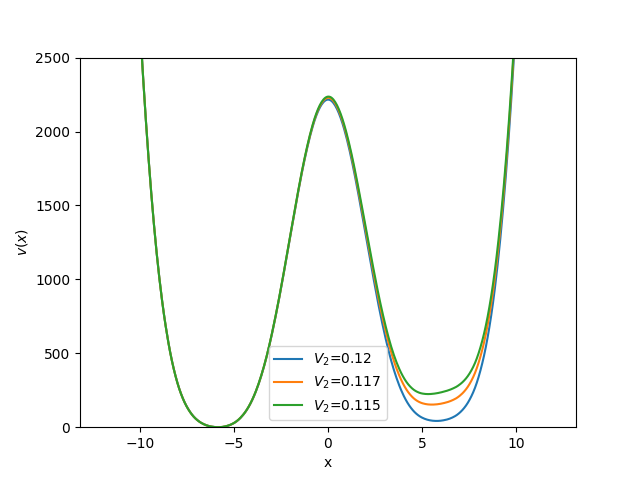
\includegraphics[scale=0.75]{figures/trap_potential.png}
\caption{ (a) Trap potential for different voltages.}
\label{fig3}
\end{figure}

\subsection{Single electron}

We use a single-particle basis (or qubit states) $\{ \phi_p \}_{p=1}^L$ that are eigenfunctions of the one-body Hamiltonian. That is, we have to solve the eigenvalue problem
\begin{equation}
   \left(-\frac{1}{2}\frac{d^2}{dx^2} + v(x)\right) \phi_p(x) = \epsilon_p \phi_p(x).
\end{equation}

We proceed by discretizing the grid and use the second-order central differences
method for the double-derivative, i.e. the finite difference method.
Building a tridiagonal matrix from the grid points, we solve the eigenvalue
equation and choose the $l$ first eigenstates (i.e., the eigenstates with the
lowest eigenenergy) as the single-particle basis $\{\psi_i\}_{i = 1}^l$.

The resulting eigenfunctions for different voltages are shown in fig.(\ref{eigenfunctions-single-particle}). Notice that the eigenfunctions are localized in the left or right well. Furthermore, as the asymmetry of the wells is increased the energies of the states in the right well increases.

Table \ref{sp-excitation-energies} gives the excitation energies/frequencies (in scaled units) between the two lowest lying states in the left and right well.  

\begin{table}
\centering
\caption{Excitation energies between the two lowest lying states in the left and right well.}
\begin{tabular}{| c | c | c | c |}
     \hline
     & $V_2 = 0.12$ & $V_2 = 0.117$ & $V_2 = 0.12$  \\
     \hline
    $\epsilon_{2_L, 1_L}$ & $8.359459$ & $8.362252$ & $8.364329$ \\
    \hline
    $\epsilon_{2_R, 1_R}$ & $8.163382$ & $7.726695$ & $7.976945$ \\
    \hline
\end{tabular}
\label{sp-excitation-energies}
\end{table}

\begin{figure}[ht]%
 \centering
 \subfloat[Eigenfunctions $V_2=0.12$]{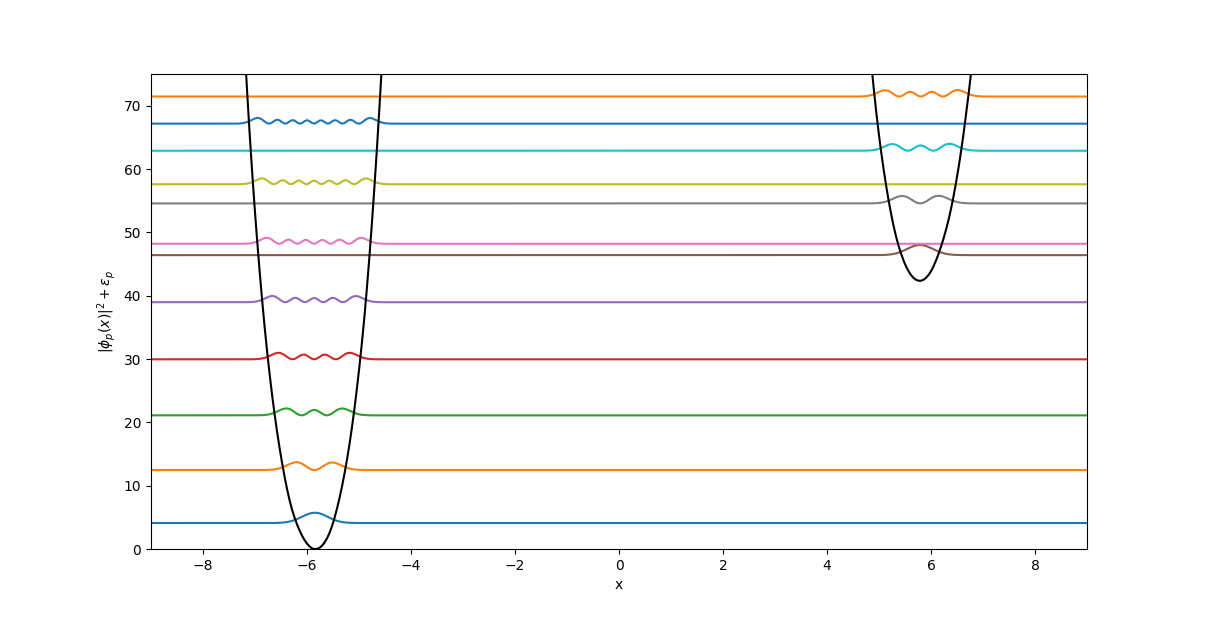
\includegraphics[scale=0.3]{figures/eigenfuncs_V2=0.12.png}\label{fig:a}}%
 \subfloat[Eigenfunctions $V_2=0.117$]{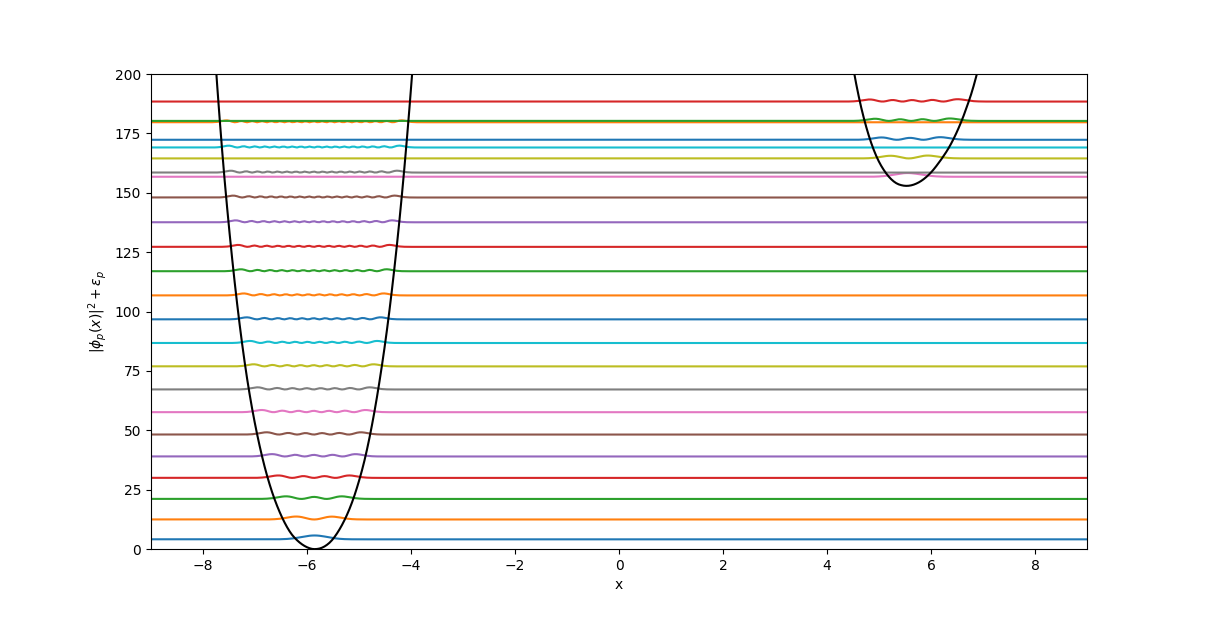
\includegraphics[scale=0.3]{figures/eigenfuncs_V2=0.117.png}\label{fig:b}}\\
 \subfloat[Eigenfunctions $V_2=0.115$]{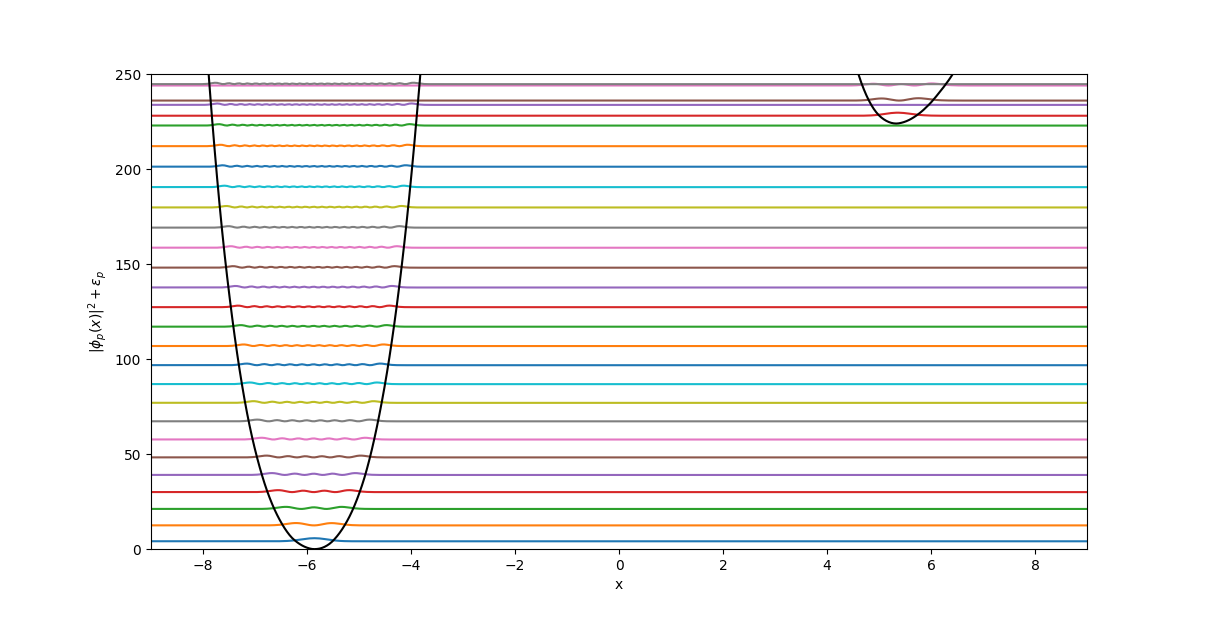
\includegraphics[scale=0.35]{figures/eigenfuncs_V2=0.115.png}\label{fig:c}}%
 \caption{Eigenfunctions for different asymmetry parameter (voltage $V_2$).}%
 \label{eigenfunctions-single-particle}%
\end{figure}

\subsection{Two non-interacting electrons}
We are interested in transition between the low-lying states. By construction, we know that the Slater determinants are eigenfunctions of the non-interacting Hamiltonian $\hat{H}_0$ if the single-particle functions are eigenfunctions of the single-particle operator. 

Fig.(\ref{SD_OBD1}) shows the one-body densities of the low-lying Slater determinants with $V_2=0.12$.

\begin{figure}
    \centering
    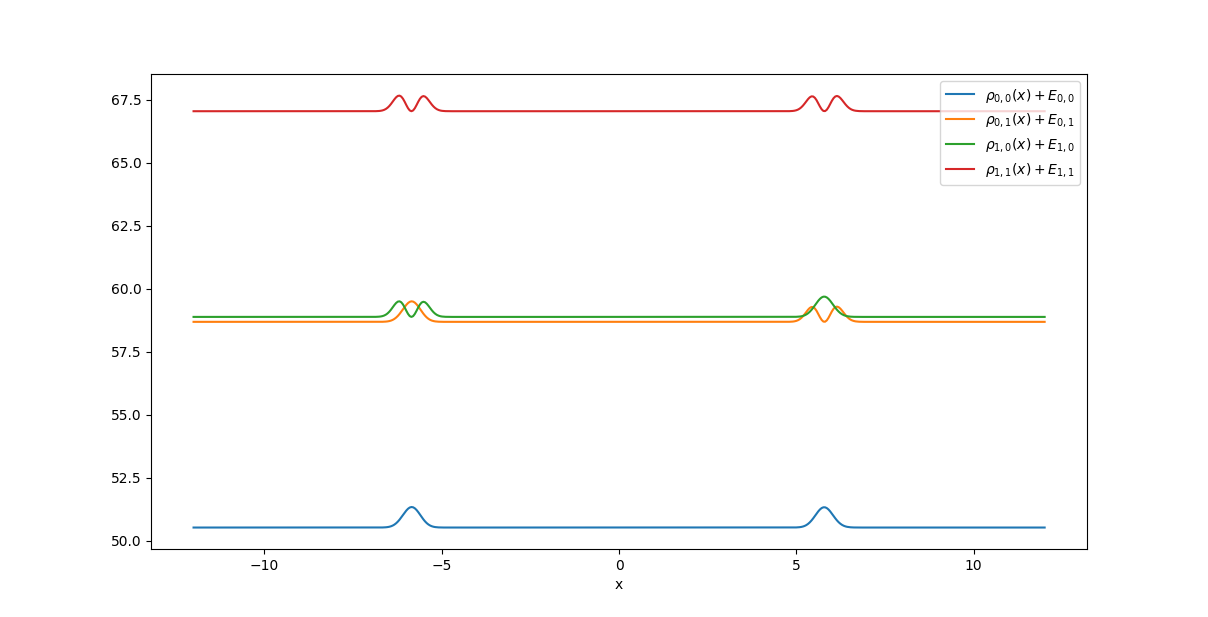
\includegraphics[scale=0.5]{figures/SD_dens_V2=0.12.png}
    \caption{One-body densities for the low-lying Slater determinants with $V_2=0.12$.}
    \label{SD_OBD1}
\end{figure}


\subsection{Two interacting electrons}

\section{Interaction with EM field}

\bibliography{apssamp}% Produces the bibliography via BibTeX.
\end{document}